\documentclass[final,hyperref={pdfpagelabels=false}]{beamer}
\mode<presentation>
{
  \usetheme{rc2018}
}
\usepackage[orientation=portrait,size=a0,scale=1.4,debug]{beamerposter}
\usepackage{multirow}


%%%%%%%%%%%%%%%%%%%%%%%%%%%%%%%%%%%%%%%%%%%%%%%%%%%%%%%%%%%%%%%%%%%%%%%%%%%%%%%%% 5
\title{Influence of inhibitory circuits on the frequency tuning of mitral cells}
\author[Miko]{Rebecca Miko, Christoph Metzner and Volker Steuber}
\institute{Biocomputation Research Group, Centre for Computer Science and Informatics Research, University of Hertfordshire, UK}
\date{Jul. 31th, 2018}

%%%%%%%%%%%%%%%%%%%%%%%%%%%%%%%%%%%%%%%%%%%%%%%%%%%%%%%%%%%%%%%%%%%%%%%%%%%%%%%%% 5
\begin{document}
\begin{frame}{} 
\begin{block}{Introduction}
Recent studies show that the structure of odour stimuli contains information about the olfactory scene \cite{celani2014odor, schmuker2016exploiting}. 
We investigated whether mitral cells (MCs) in the olfactory bulb (OB) can show frequency tuning and, if they do, how different components of the glomerular layer circuitry  shape and determine the tuning.
\end{block}    
\begin{columns}[t]
\begin{column}{.48\linewidth}

\begin{block}{Model} 
\begin{figure}
\centering
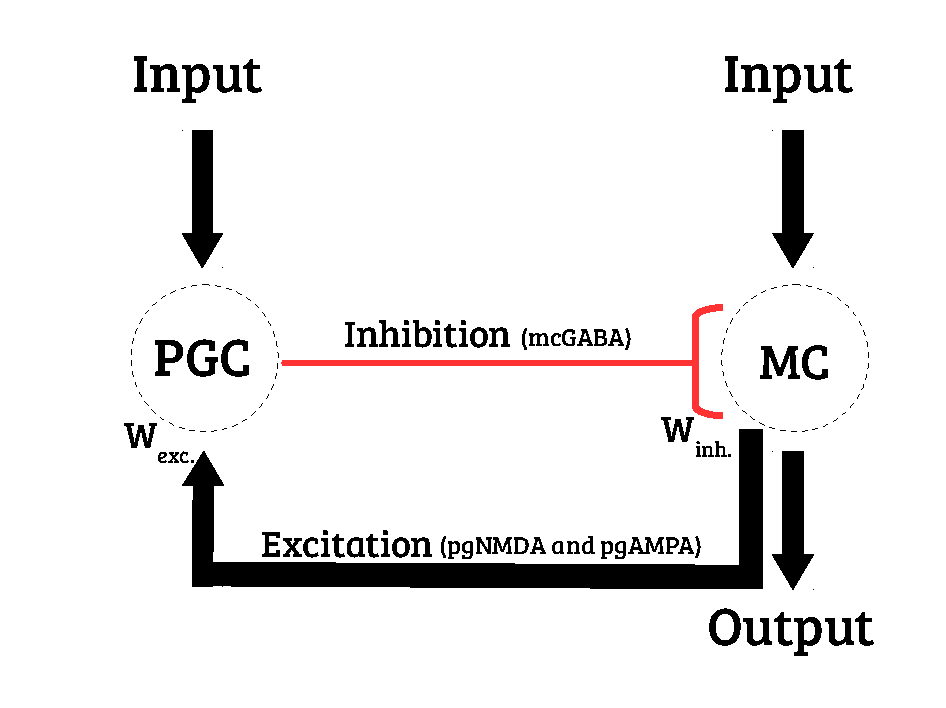
\includegraphics[scale=1.3]{poster_images/Circuit_Diagram}
\end{figure}
\begin{itemize}
\item We used a model of the OB (modified from \cite{li2013two}).
\item Modeled MC-PGC (periglomerular cells), focusing on recurrent and feed - forward inhibition in the glomerular layer.
\end{itemize}
\end{block}

\begin{block}{Method} 
\begin{itemize}
\item Parameter combinations: PGC input strength, MC-PGC excitation strength and PGC-MC inhibition strength.
\item We used sinusoidal currents of varying frequencies as input, using the equation:\\
\end{itemize}

\[
\text{y(t) = c\cdot sin(2} \pi \text{f}\cdot \text{t + } \varphi\text{) + 0.18}
\]
\begin{itemize}
\item Where c = 0.45nA (strength of input to MC) and $\text{\varphi}$ = 0 (phase).
\item PGC input is defined as i\cdot c, where i is the PGC input factor.
\end{itemize}
\begin{center}
\begin{tabular}{ c c c c c c  }
\hline 
\multirow{2}{*}{Parameter} & \multicolumn{5}{c}{\multirow{2}{*}{Iteration Values}}\\
\multirow{2}{*}{} & \multirow{2}{*}{} & \multirow{2}{*}{} & \multirow{2}{*}{} & \multirow{2}{*}{} & \multirow{2}{*}{}\\
\hline
\multirow{2}{*}{PGC Input Factor (i)} & \multirow{2}{*}{0.2,} & \multirow{2}{*}{0.3,} & \multirow{2}{*}{0.4,} & \multirow{2}{*}{0.5,} & \multirow{2}{*}{0.6} \\ 
\multirow{2}{*}{} & \multirow{2}{*}{} & \multirow{2}{*}{} & \multirow{2}{*}{} & \multirow{2}{*}{} & \multirow{2}{*}{}\\
\hline
\multirow{2}{12em}{\centering MC-PGC Excitation Strength (\mbox{$\text{W}_{\text{exc}}$})} & \multirow{2}{*}{2.0,} & \multirow{2}{*}{4.0,} & \multirow{2}{*}{6.0,} & \multirow{2}{*}{8.0,} & \multirow{2}{*}{10.0}  \\
\multirow{2}{*}{} & \multirow{2}{*}{} & \multirow{2}{*}{} & \multirow{2}{*}{} & \multirow{2}{*}{} & \multirow{2}{*}{}\\
\hline
\multirow{2}{12em}{\centering PGC-MC Inhibition Strength (\mbox{$\text{W}_{\text{inh}}$})} & \multirow{2}{*}{1.0,} & \multirow{2}{*}{2.0,} & \multirow{2}{*}{3.0,} & \multirow{2}{*}{4.0,} & \multirow{2}{*}{5.0} \\
\multirow{2}{*}{} & \multirow{2}{*}{} & \multirow{2}{*}{} & \multirow{2}{*}{} & \multirow{2}{*}{} & \multirow{2}{*}{}\\
\hline
\multirow{2}{*}{Frequency (f)} & \multirow{2}{*}{1.0,} & \multirow{2}{*}{2.0,} & \multirow{2}{*}{3.0,} & \multirow{2}{*}{... ,} & \multirow{2}{*}{40.0}\\
\multirow{2}{*}{} & \multirow{2}{*}{} & \multirow{2}{*}{} & \multirow{2}{*}{} & \multirow{2}{*}{} & \multirow{2}{*}{}\\
\hline
\end{tabular}
\end{center}
\begin{itemize}
\item Constructed frequency tuning curves and then extracted the peak resonance frequency.
\end{itemize}
\begin{figure}
\centering
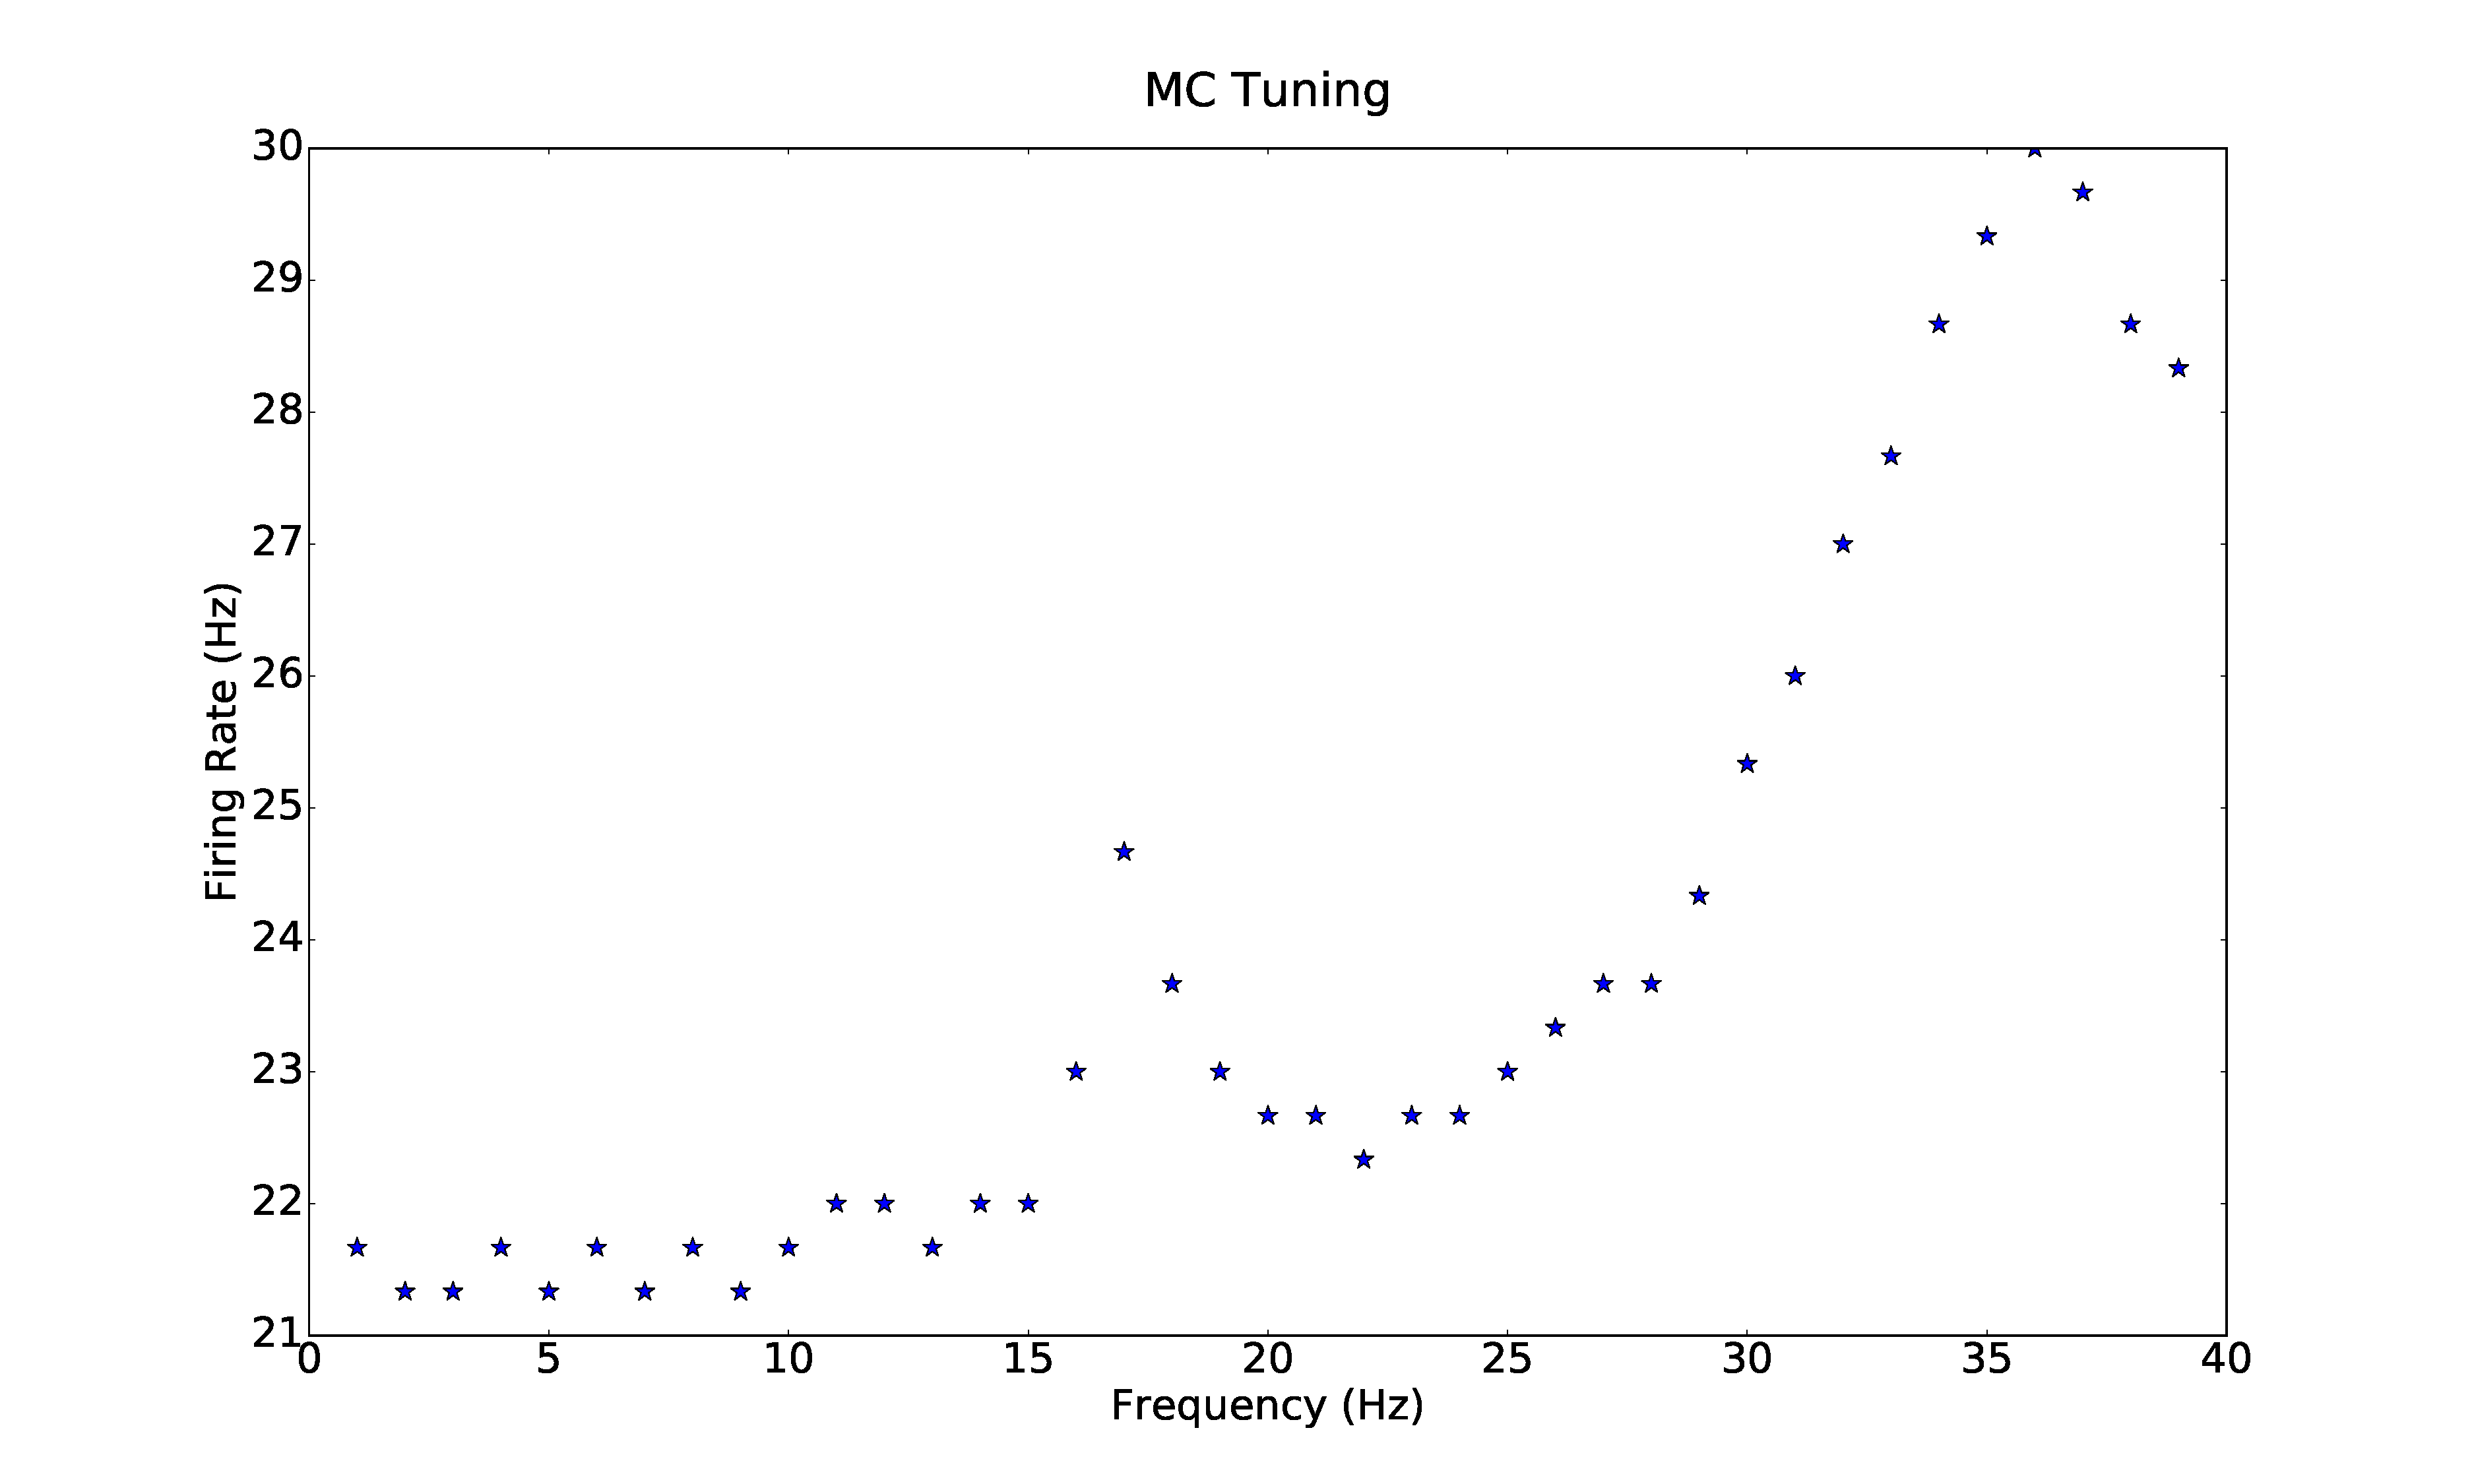
\includegraphics[scale=0.55]{poster_images/Figure3}
\end{figure}
\begin{itemize}
\item Extracted the resonance strength of the tuning Q, measured as: \\
\end{itemize}

\[
\text{Q =} \frac{\text{(F}_{\text{max}} \text{-F}_{\text{min}}\text{)}}{<\text{F}>}
\]
\begin{itemize}
\item \mbox{$\text{F}_{\text{max}}$} and \mbox{$\text{F}_{\text{min}}$} are maximum and minimum firing rate.
\item $<$F$>$ is mean firing rate over all measured frequencies.
\end{itemize}
\end{block}

\end{column}
\begin{column}{.48\linewidth}

\begin{block}{Results}
\begin{figure}
\centering
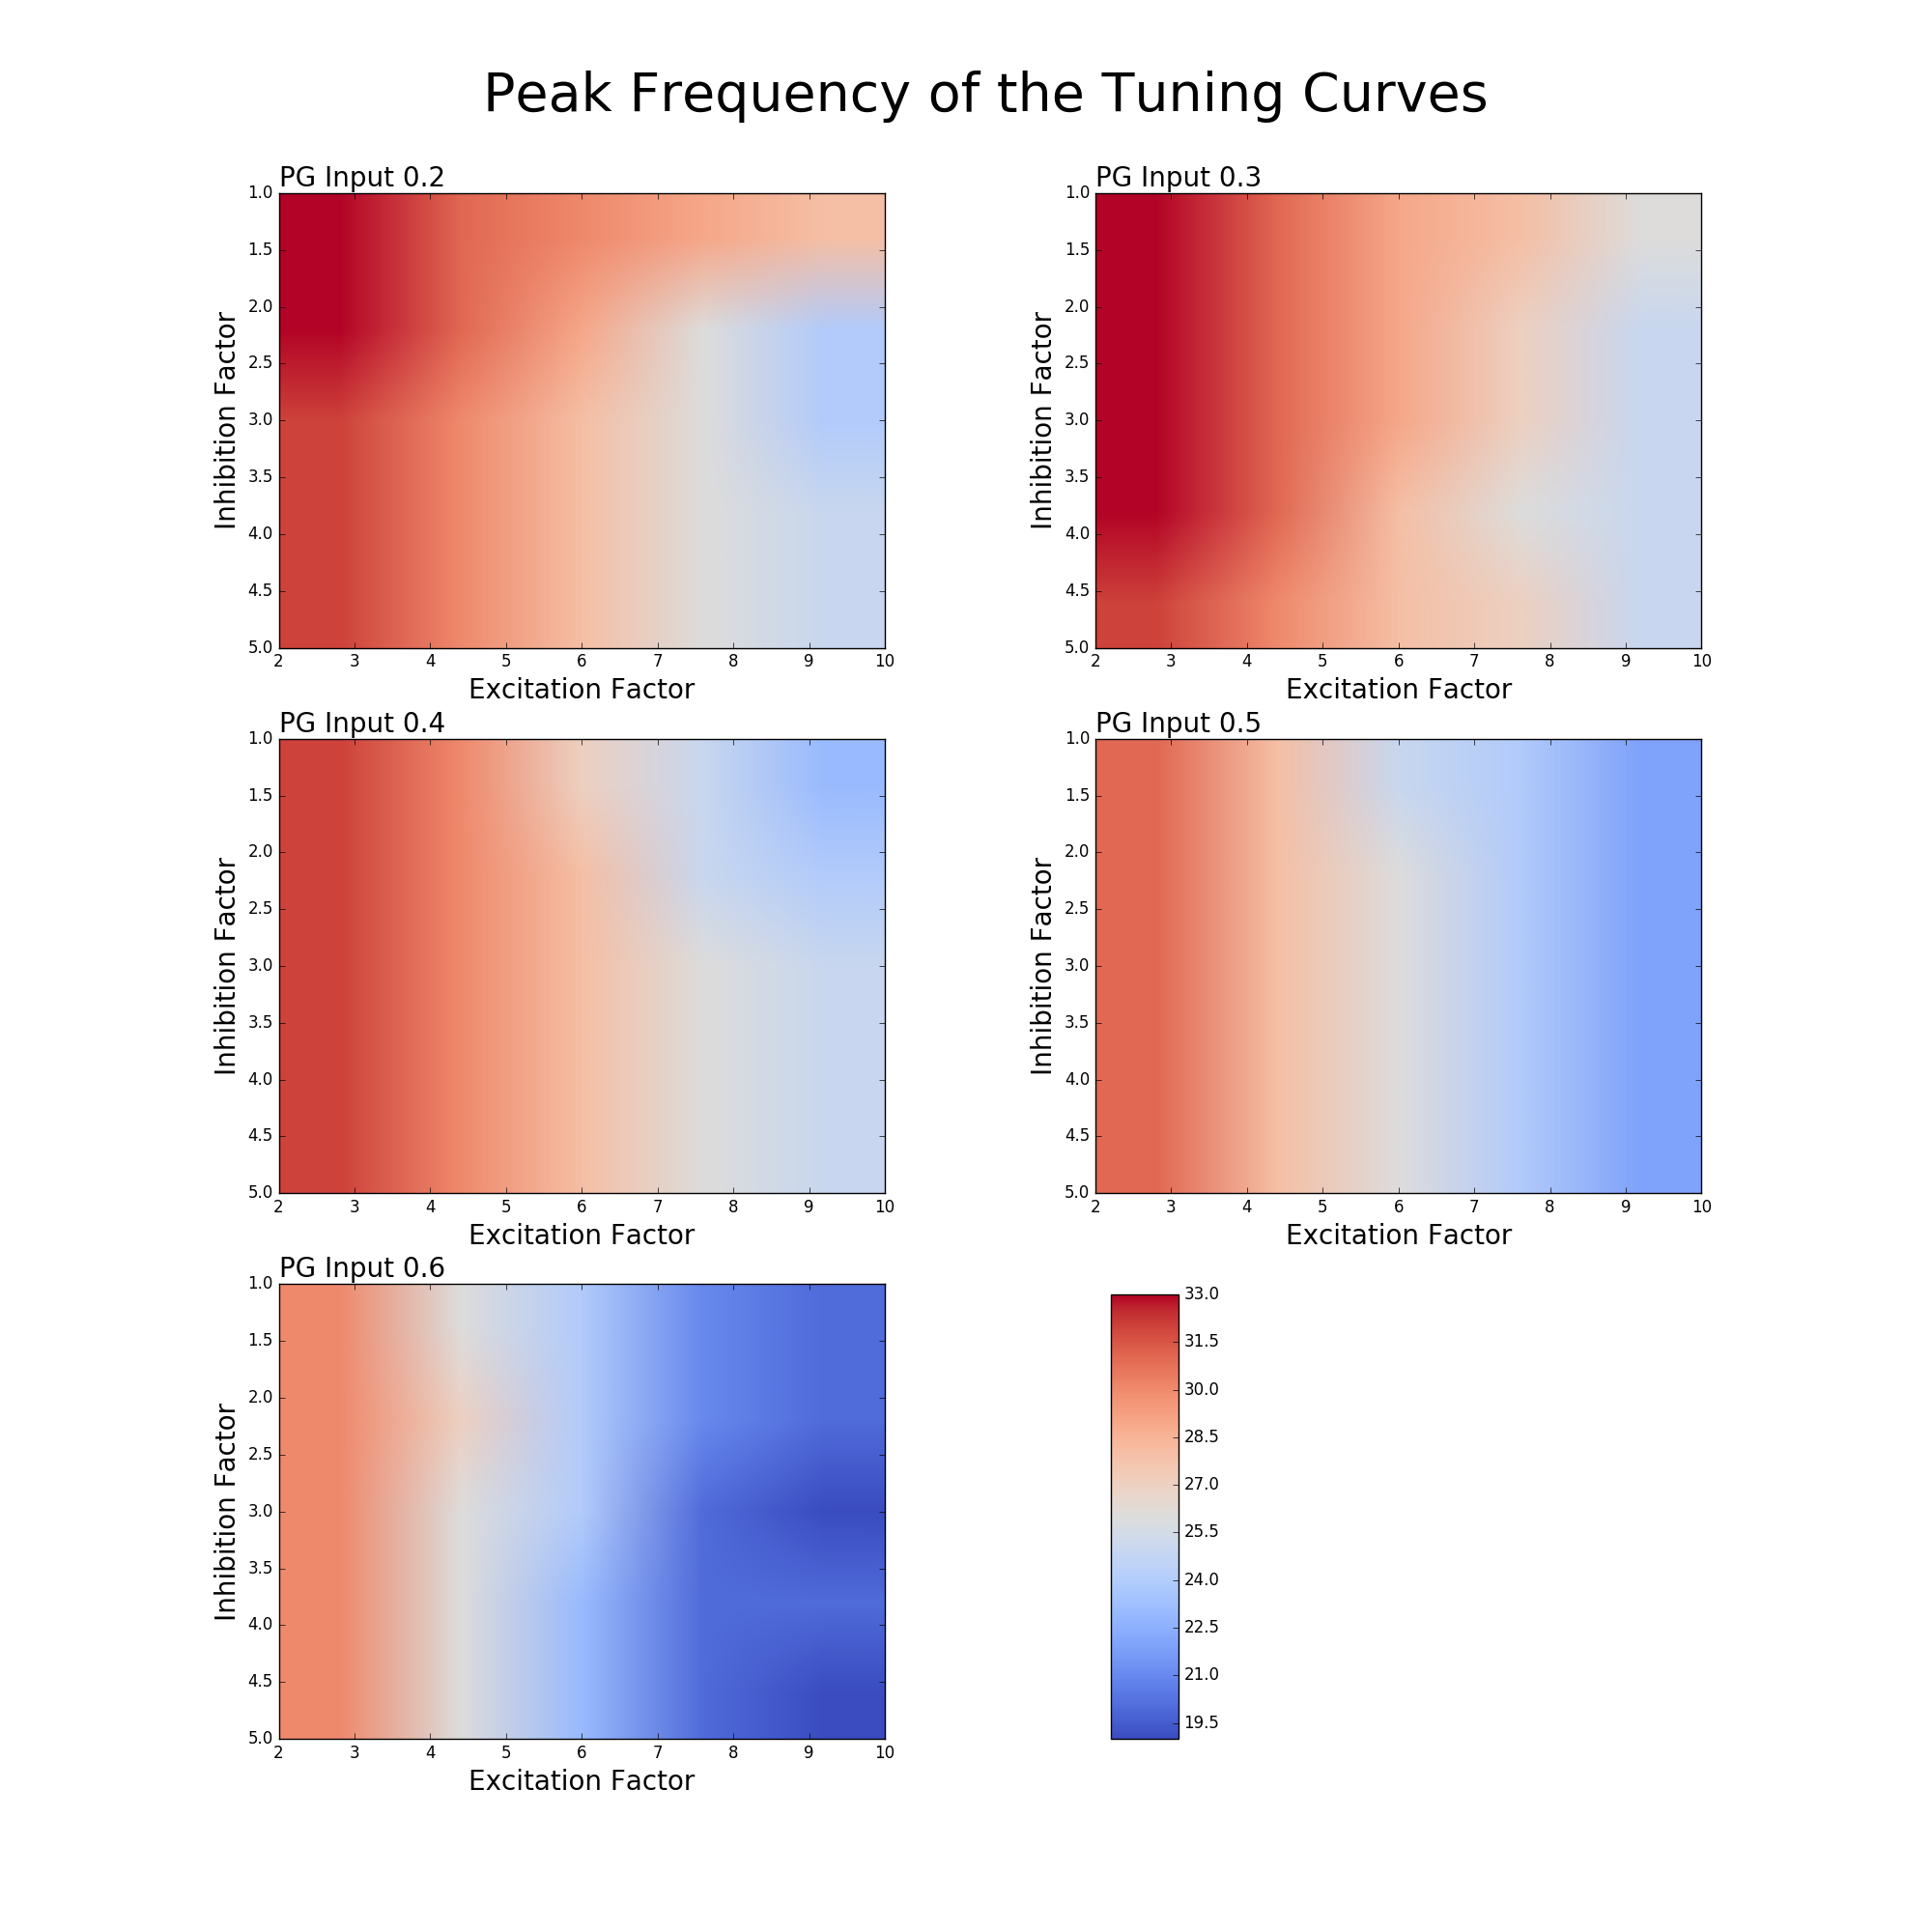
\includegraphics[scale=0.6, trim = 0 17cm 0 0, clip]{poster_images/Contour_plot_tuning_frequency}
\end{figure}
\begin{itemize}
\item Resonance frequency decreased as the excitation of the PGC increased (both from input and the MC).
\item Strength of PGC inhibition onto the MC did not have a strong effect.
\end{itemize}
\begin{figure}
\centering
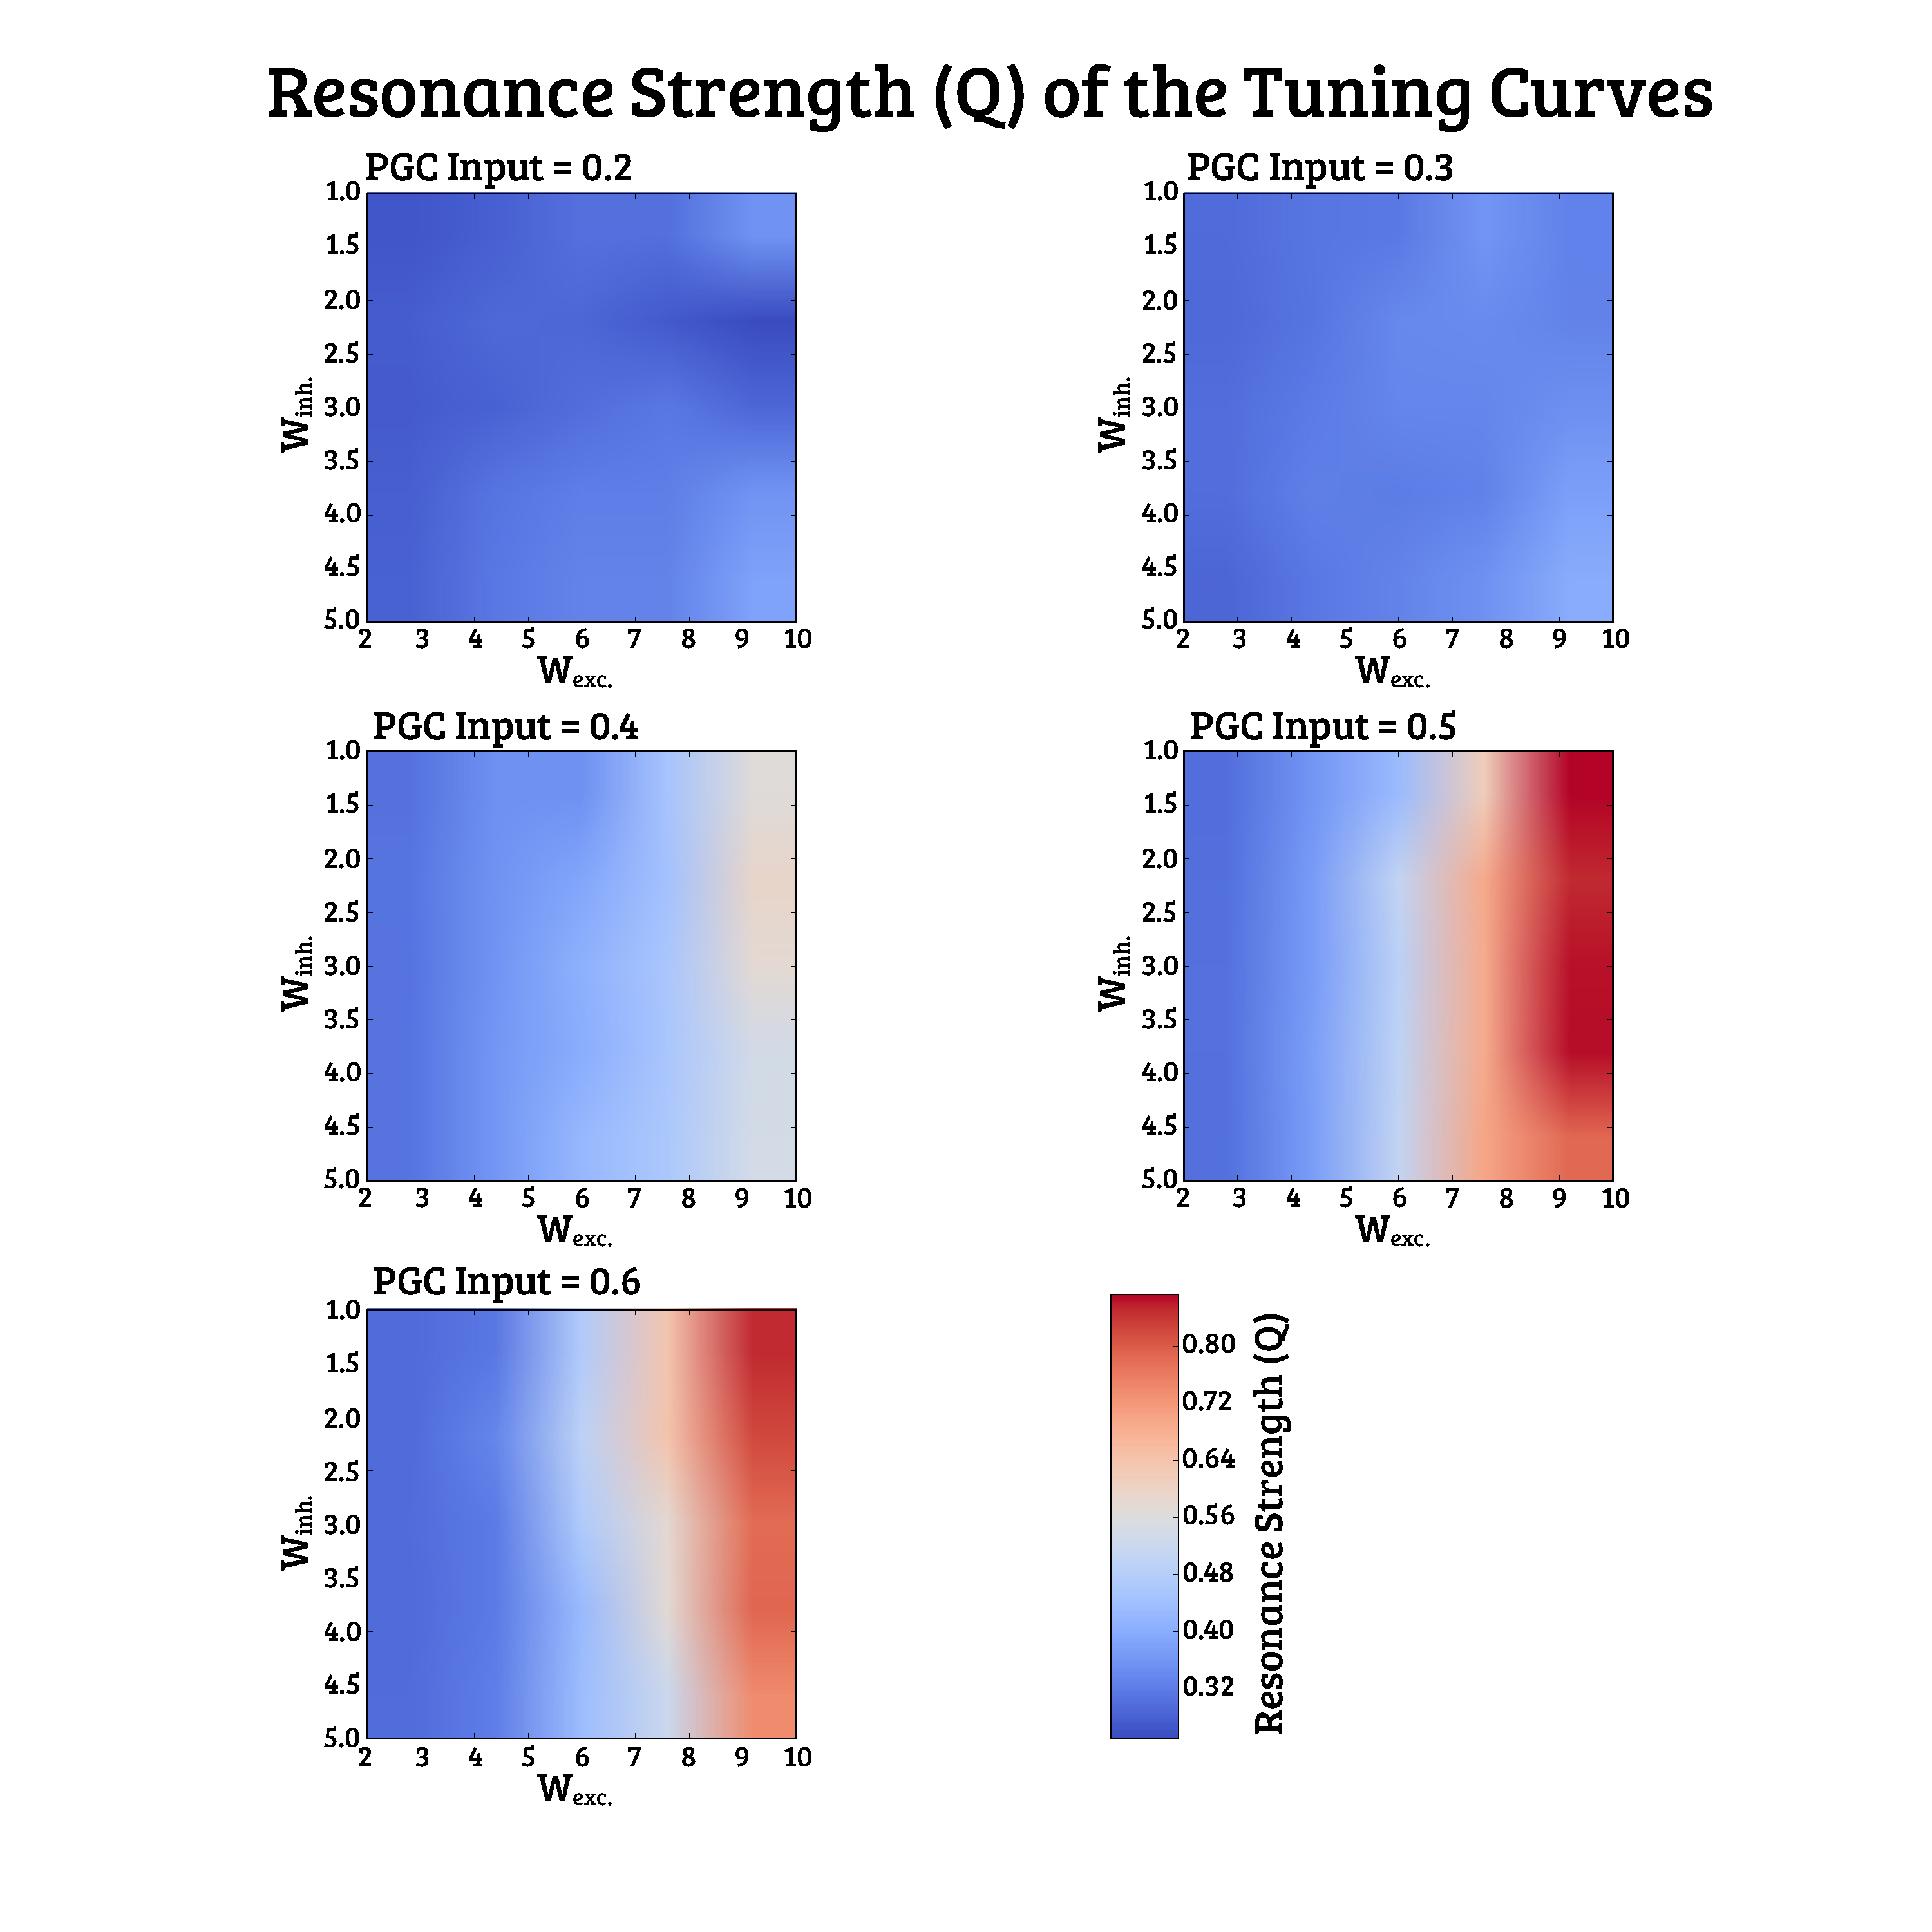
\includegraphics[scale=0.6, trim = 0 17cm 0 0, clip]{poster_images/Contour_plot_tuning_strength}
\end{figure} 
\begin{itemize}
\item Resonance strength increased with the strength of the excitatory connection, when the PGC received sufficient external input.
\end{itemize}
\end{block}

\begin{block}{Conclusion}
\begin{itemize}
\item Our results suggest that MCs can show frequency tuning in the presence of sufficiently strong excitatory connections between MCs and PGCs, which provide feedback inhibition to the MCs.
\item Therefore, the OB might be able to detect the frequency composition of signals.
\item This could be used for olfactory scene analysis.
\item However, we only see tuning in a narrow frequency range.
\end{itemize}
\end{block}

\begin{block}{Acknowledgements} 
We thank Michael Schmuker for his comments and support.
\end{block}

\begin{block}{References}
\nocite{*}
\bibliographystyle{plain}
{\footnotesize
\bibliography{BibList}
}
\end{block}

\end{column}
\end{columns}

\end{frame}
\end{document}

%%%%%%%%%%%%%%%%%%%%%%%%%%%%%%%%%%%%%%%%%%%%%%%%%%%%%%%%%%%%%%%%%%%%%%
